\documentclass[a4paper]{article}

\usepackage[utf8]{inputenc}
\usepackage[T1]{fontenc}
\usepackage[francais]{babel}
\usepackage[top=1.5cm, left=2.5cm, bottom=1.5cm, right=2.5cm]{geometry}
\usepackage{amsmath}
\usepackage{amssymb}
\usepackage{textcomp}
\usepackage{graphicx}

\author{Théo Verhelst}
\title{Matière non-exhaustive pour l'examen du cours de Modélisation et
Simulation}

\begin{document}
\maketitle
\tableofcontents
\section{Introduction}
Ce document reprend les questions/définitions listées par Mr. Bontempi comme
étant des questions potentielles à son examen oral, et y répond à partir du
contenu du syllabus.\\
Sont reprises également quelques autres notions importantes tirées du cours.
\paragraph{}
\emph{Note :} Toutes les définitions ne sont pas explicitées formellement, car
Mr. Bontempi m'a assuré que seul la compréhension des concepts est évaluée, pas
la restitution pure des définitions.
\paragraph{}
\emph{Note 2 :} Les variables et conventions de notation utilisées sont basées
sur celles du syllabus.
\section{Définitions}
\subsection{Propriétés de la fonction de transition}
\begin{itemize}
	\item \emph{Consistance :} Si l'état du système au temps $t$ est $x$,
		la fonction de transition à l'instant $t$ doit donner $x$.
		\[\varphi(t,t,x,u(\cdot))=x\quad\forall t\in T, x\in X,
		u(\cdot)\in\Omega\]
	\item \emph{Irreversibilité :} $\varphi$ est définie pour tout
		\(t \ge t_0, t\in T\)
	\item \emph{Composition :} Si l'entrée $u(\cdot)$ fait évoluer l'état de
		$x_0$ à $\varphi(t_2,t_0,x_0,u(\cdot))$ durant $[t_0,t_2]$ en passant
		par $x(t_1)$, alors la même entrée fera passer l'état de $x(t_1)$ à
		$\varphi(t_2,t_0,x_0,u(\cdot))$ durant $[t_1,t_2]$.
	\item \emph{Causalité :} Si deux fonction d'entrées sont identiques sur un
		intervalles, elles auront le même effet dans cette intervalle sur un
		système donné pour un état initial donné.
\end{itemize}
\subsection{Accessibilité}
Un état $x_2$ est \emph{accessible} à l'instant $t_2$ à partir d'un état $x_1$
si $\exists\;t_1, u(\cdot)$ tels que \[\varphi(t_2,t_1,x_1,u(\cdot))=x_2\]
\subsection{Observabilité}
\subsection{Notions de stabilité}
Un système est dit  \emph{stable} si une petite perturbation de son état initial
n'induit pas une grande perturbation de son comportement au cours du temps.\\
Plus formellement, un mouvement avec une condition initiale $\bar x$ est
stable si pour tout voisinage $V_\epsilon$ de ce mouvement, on peut trouver
une condition initale proche de $\bar x$ telle que le mouvement partant de
cette condition initiale perturbée reste dans le voisinage $V_\epsilon$.
\subsection{Critère de stabilité de Liapounov}
Soit un système à temps continu
\[\dot x(t)=f(x(t),u(t))\]
où le vecteur de fonctions $f(\cdot, \cdot)$ est continu ainsi que ses
dérivées partielles.\\
Soit $\bar x$ un état d'équilibre pour la fonction d'entrée constante $\bar u$.
\begin{itemize}
	\item \emph{Critère de stabilité de Liapounov :} S'il existe une fonction
		$V(\cdot)$ continue (et que ses dérivées partielles sont également
		continues), qui soit définie positive en $\bar x$ et telle que sa
		dérivée par rapport au temps soit semi-définie négative en $\bar x$,
		alors $\bar x$ est un état d'équilibre stable.
		Avec
		\[
			\dot V(x)=\frac{dV(x)}{dt}
			=\langle\Delta V(x),\,f(x,\bar u)\rangle
			=\sum_{i=1}^{n}\frac{\partial V}{\partial x_i}\dot x_i(t)\]
		où le gradient de \(V\) est
		\[\Delta V(x)=\big[\frac{\partial V}{\partial x_1},\dots
		\frac{\partial V}{\partial x_n}\big]\]
		et où \(\langle\cdot,\,\cdot\rangle\) désigne le produit scalaire.
	\item \emph{Critère de stabilité asymptotique de Liapounov :}
		Si le critère de stabilité de Liapounov est satisfait et que
		$\dot V(\cdot)$ est définie négative (et non uniquement semi-définie
		négative) en $\bar x$, alors $\bar x$ est asymptotiquement stable.\\
		Dans ce cas, une telle fonction \(V\) est appelée fonction de Liapounov.
	\item \emph{Critère d'instabilité de Liapounov :} Même restrictions
		que pour le critère de stabilité de Liapounov, si ce n'est que
		$\dot V(\cdot)$ doit être définie positive, et non
		(semi-)définie négative. Si c'est le cas, alors \(\bar x\) est
		un état d'équilibre instable.
\end{itemize}
\subsection{Propriétés des systèmes linéaires continus}
Définissons d'abord deux notions sur les mouvements:
\begin{itemize}
	\item Le \emph{mouvement libre} est obtenu quand la fonction d'entrée est
		nulle ($u(\cdot)=0$).
	\item Le \emph{mouvement forcé} est obtenu quand la l'état initial est nul
		($x(t_0)=0$).
\end{itemize}
Un système linéaire jouit des propriétés suivantes:
\begin{itemize}
	\item Tout mouvement est la somme des mouvements libre et forcés
		correspondants.
	\item Si l'état initial $x_0$ est une combinaison linéaire
		$ax_{01} + bx_{02}$ de deux états initiaux, alors le mouvemement libre
		correspondant est la même combinaison linéaire des deux mouvemements
		libres correspondant à $x_{01}$ et $x_{02}$.
	\item Si la fonction d'entrée $u(\cdot)$ est une combinaison linéaire
		$au_1(\cdot) + bu_2(\cdot)$ de deux fonctions d'entrée, alors le
		mouvemement forcé correspondant est la même combinaison linéaire des
		deux mouvemements forcés correspondant à $u_1(\cdot)$ et $u_2(\cdot)$.
	\item La transformation de sortie $\eta$ est une fonction linéaire.
\end{itemize}
\subsection{Relation entre stabilité et le critère de Hurwitz}
Satisfaire le critère de Hurwitz est équivalent à prouver que le système
est asymptotiquement stable.\\
Le citère de Hurwitz se formulle comme suit:\\
Soit le système linéaire invariant et autonome
\[\dot x(t)=Ax(t)\]
et soit
\[\Delta_A(\lambda)=det(\lambda I - A)
= \lambda^n+\sum_{i=1}^na_i\lambda^{n-i}\]
son polynôme caractéristique. Posons
\[H=\begin{bmatrix}
	a_1 & 1 & 0 & 0 & \dots \\
	a_3 & a_2 & a1 & 1 & \dots \\
	a_5 & a_4 & a_3 & a_2 & \dots \\
	a_7 & a_6 & a_5 & a_4 & \dots \\
	\vdots & \vdots & \vdots & \vdots & \\
\end{bmatrix}
\]
où $a_{n+i} = 0\quad\forall i > 0$.\\
Le critère de Hurwitz est satisfait si tous les mineurs principaux de $H$ sont
positifs.
\subsection{Solutions générale d'un système linéaire du second ordre}
Soit le système
\[\dot x=Ax\Leftrightarrow
	\begin{cases}
		\dot x_1 = a_{11}x_1 + a_{12}x_2\\
		\dot x_2 = a_{21}x_1 + a_{22}x_2
	\end{cases}
\]
Les valeurs propres de la matrice \(A\) sont les solutions \(\lambda_{1,2}\) de l'équation
\[det(\lambda I-A)=0\]
En développant, on a
\[\lambda_{1,2} = \frac{a_{11}+a_{22} \pm \sqrt{(a_{11}+a_{22})^2 - 4(a_{11}a_{22} - a_{12}a_{21})}}{2}
	=\frac{tr(A)\pm\sqrt{tr^2(A) - 4det(A)}}{2}
\]
Les vecteurs propres \(v_{1,2}\) associés aux valeurs propres \(\lambda_{1,2}\) sont définis par
\[\begin{cases}
	\lambda_1 v_1=Av_1\\
	\lambda_2 v_2=Av_2
\end{cases}\]
En développant, on peut trouver, \(\forall\, i\in\{1, 2\}\)
\[v_i=\begin{bmatrix}
	\frac{a_{12}}{\lambda_i - a_{11}}\\
	1
\end{bmatrix}
\]
La solution générale du système est une combinaison linéaire de fonctions
exponentielles caractérisée par ces valeurs et vecteurs propres, ainsi que par
deux constantes \(c_{1,2}\) déterminées par les conditions initiales:
\[x(t)=c_1 v_1 e^{\lambda_1 t} + c_2 v_2 e^{\lambda_2 t}\]
\[\Leftrightarrow
\begin{cases}
	\dot x_1 = c_1 \left( \frac{a_12}{\lambda_1-a_{11}}\right) e^{\lambda_1 t} +
	           c_2 \left( \frac{a_12}{\lambda_1-a_{11}}\right) e^{\lambda_1 t} \\
	\dot x_2 = c_1 e^{\lambda_1 t} + c_2 e^{\lambda_2 t}
\end{cases}
\]
\subsection{Principe de superposition des effets dans le cas d'un système
linéaire du second ordre}
\emph{Note:} je ne sais pas très bien ce qu'il veut qu'on dise à propos de ce
point, étant donné qu'un système linéaire satisfait, par définition, les
critères du principe de superposition des effets.
\paragraph{}
Soit le système
\[
	\begin{cases}
		\dot x(t)&= A(t)x(t) + B(t)u(t)\\
		y(t)&=C(t)x(t)
	\end{cases}
\]
où \(A,\,B,\,C\) sont des matrices \(2\times 2\) de fonctions continues en
\(T\). Alors, par le théorème 5.2 du syllabus, ce système est linéaire, et donc
satisfait les critères du principe de superposition des effets.
\subsection{Classifier la stabilité des systèmes de seconde ordre par rapport à
la matrice des coefficients}
Soit le système
\[\dot x=Ax\Leftrightarrow
\begin{bmatrix}
	\dot x_1\\
	\dot x_2
\end{bmatrix}
=
\begin{bmatrix}
	a_{11} & a_{12}\\
	a_{21} & a_{22}
\end{bmatrix}
\begin{bmatrix}
	x_1\\
	x_2
\end{bmatrix}
\]
Soient \(\lambda_1, \lambda_2\in\mathbb{C}\) les valeurs propres de la matrice \(A\).\\
On peut alors dire que
\begin{itemize}
	\item Le système est asymptotiquement stable si et seulement si
		\[\Re(\lambda_i) < 0\quad\forall\, i\in\{1, 2\}\]
	\item Le système est simplement stable si et seulement si
		\begin{align*}
			&\Re(\lambda_i) \le 0 \\
			\land\,&
			((\Re(\lambda_i) = 0) \Rightarrow \lambda_i \text{ est de multiplicité } 1)
			\quad\forall\, i\in\{1, 2\}
		\end{align*}
	\item Le système est instable dans tous les autres cas, c'est à dire si et seulement si
		\begin{align*}
			&\exists i\in\{1, 2\} \text{ t.q. } \Re(\lambda_i) > 0 \\
			\lor\,&
			\exists i\in\{1, 2\} \text{ t.q. } \lambda_i \text{ est de multiplicité} > 1
		\end{align*}
\end{itemize}
De plus, soient
\[tr(A)=a_{11} + a_{22}\]
\[det(A)=a_{11}a_{22} - a_{12}a_{21}\]
On peut également classer les systèmes en fonction de leur trace et de leur
déterminant:\\
\\
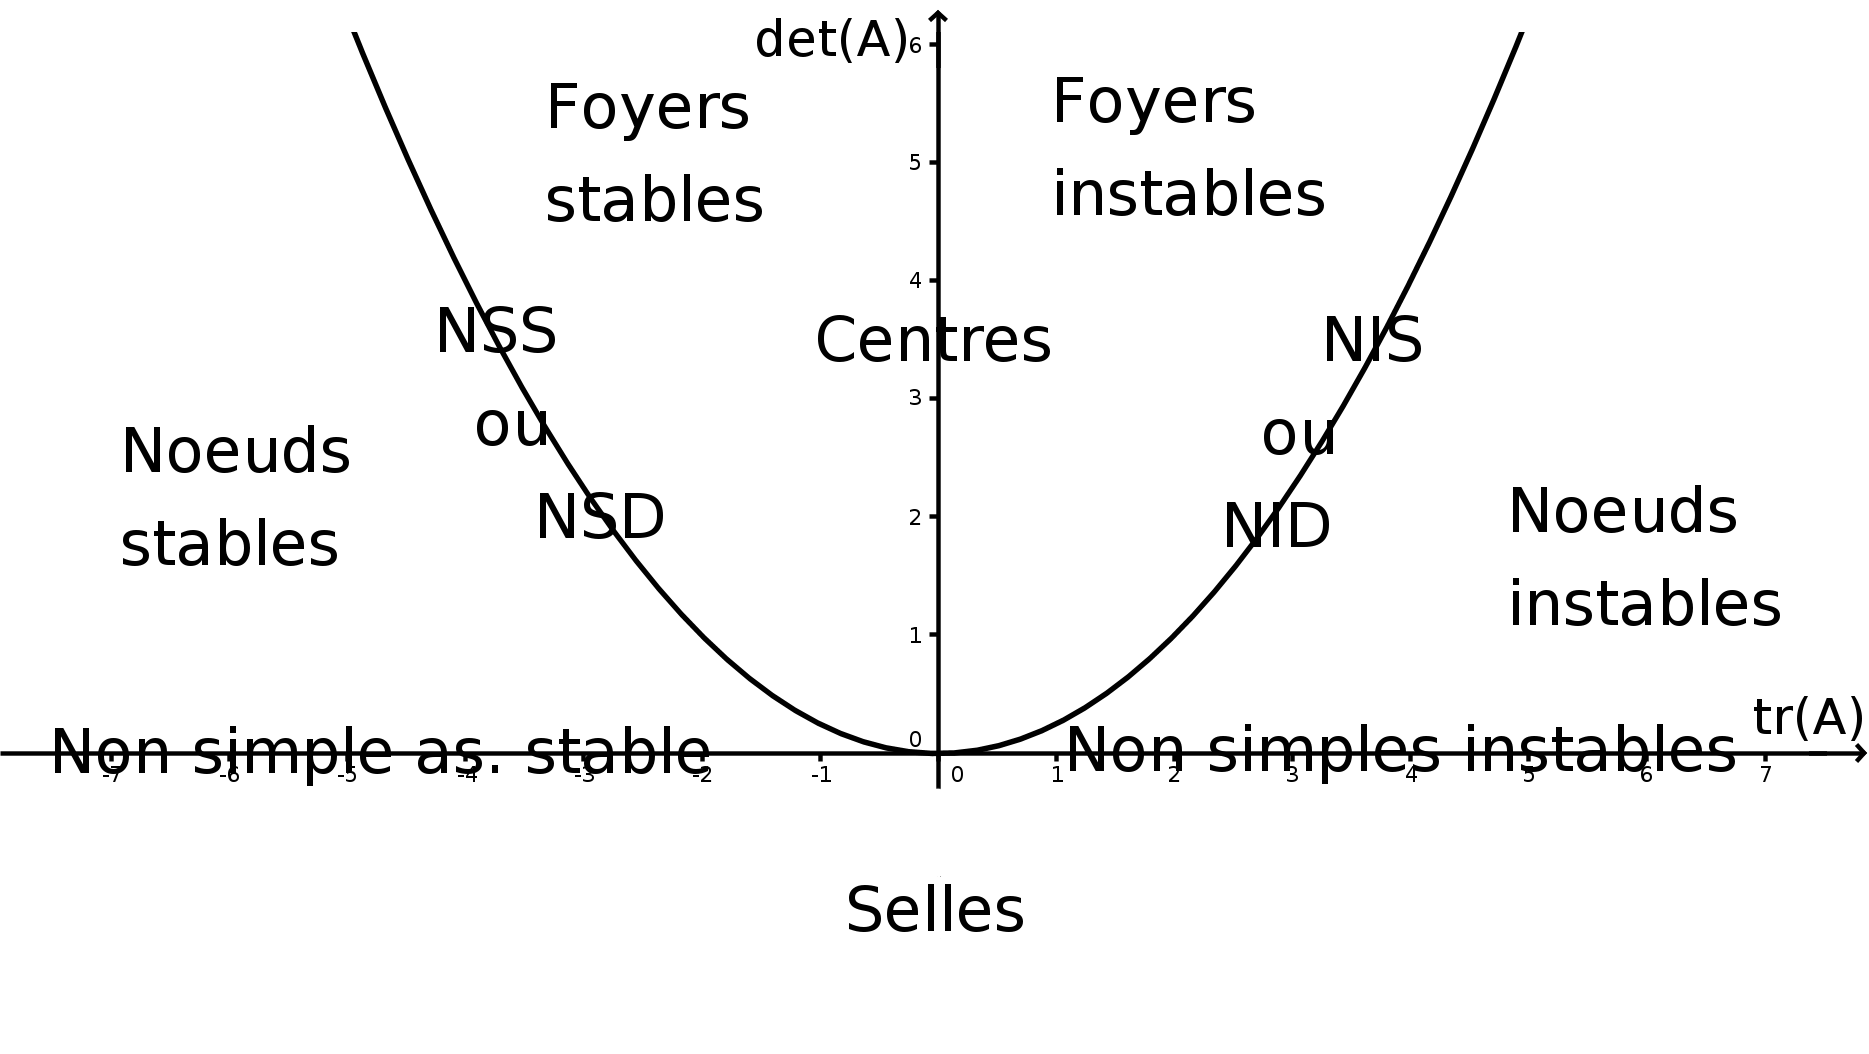
\includegraphics{graphic.png}\\
\begin{description}
	\item[NSS]: noeuds stables singuliers
	\item[NSD]: noeuds stables dégénérés
	\item[NIS]: noeuds instables singuliers
	\item[NID]: noeuds instables dégénérés
\end{description}
La parabole des noeuds singuliers ou dégénérés est d'équation
\[det(A)=\frac{(tr(A))^2}{4}\]
\subsection{Relation entre linéarisation et stabilité}
Soit le système
\[\dot x=f(x,u)\]
avec un point d'équilibre \(\bar x\) et sa linéarisation en \(\bar x,\bar u\)
\[
	\dot x=\left. \frac{\partial f}{\partial x}\right|_{\bar x,\bar u}x
	+\left. \frac{\partial f}{\partial u}\right|_{\bar x,\bar u}u
	=Ax+Bu
\]
\begin{itemize}
	\item Si le système linéarisé est asymptotiquement stable
		(c'est-à-dire toutes les valeurs propres de \(A\) sont négatives),
		alors l'état d'équilibre \(\bar x\) est asymptotiquement stable.
	\item Si la matrice \(A\) du système linéarisé a une ou plusieurs valeurs
	propres avec partie réelle positive, alors l'état d'équilibre \(\bar x\)
	du système est instable.
\end{itemize}
\subsection{Notion de diagramme de bifurcation}
Dans le cadre d'un système paramétrique continu d'ordre 1, un diagramme
de bifurcation est un graphique représentant la position des points fixes
du système (en ordonnée) en fonction du paramètre (en abscisse).
\subsection{Cycle limite}
Un cycle limite est une trajectoire fermée et isolée. Isolée veut dire
que les trajectoire avoisinantes ne sont pas closes.\\
Un cycle limite peut être stable (ou attracteur), instable ou demi-stable.
Ce dernier cas représente un cycle limite dont les trajectoires intérieures
(exterieures) convergent, alors que les trajectoires exterieures (intérieures)
divergent.
\subsection{Dimensionnalité d'un ensemble fractal}
Pour une courbe ou une surface fractale créée par un processus de
fragmentation avec \(N\) copies de taille \(r\), la \emph{dimension
fractale} \(D_0\) (ou \emph{dimension de Hausdorff}) de cette courbe est:
\[D_0=\frac{\log N}{\log r^{-1}}\]
\subsection{Système chaotique}
Un comportement chaotique est un comportement apériodique à long terme
d'un système déterministe qui affiche une sensible dépendance aux
conditions initiales.\\
Un système chaotique est un système dont le comportement est chaotique.
\subsection{Équation caractéristique et solutions d'un système linéaire à temps
discret}
Soit le système
\[x(k+n)+\sum_{i=0}^{n-1}a_i(k)x(k+i)=g(k)\]
L'équation homogène associée est
\[x(k+n)+\sum_{i=0}^{n-1}a_i(k)x(k+i)=0\]
L'équation caractéristique associée à l'équation homogène est
\[\lambda^n+\sum_{i=0}^{n-1}\lambda^ia_i=0\]
Pour toute solution \(\lambda\) de multiplicité \(m\) de l'équation
caractéristique, on a
\[x^{(i)}(k)=k^i\lambda^k\quad 0\le i<m\]
\(m\) solutions linéarement indépendantes de l'équation homogène.\\
Toute solution de l'équation homogène peut s'écrire sous la forme
\[x^{(h)}=\sum_{i=0}^{n-1}c_ix^{(i)}(k)\]
où les \(x^{(i)}(k)\) sont \(n\) solutions linéairement indépendantes de
l'équation homogène, et les constantes \(c_i\) sont déterminées
arbitrairement, ou en fonction des conditions initiales. \\
Soit \(x^{(p)}(k)\) une solution particulière de l'équation non-homogène.
Toute solution générale de l'équation non-homogène est de la forme
\[x(k)=x^{(p)}(k)+x^{(h)}(k)\]
\subsection{Étude graphique d'une équation linéaire affine à un pas}
Soit le système
\[x(k+1)=f(x(k))\]
On peut représenter son évolution avec un graphique ayant comme axes
\(0_{x'}\equiv x(k)\) en abscisse, et \(0_{y'}\equiv x(k+1)=f(x(k))\) en ordonnée.\\
En traçant dans cet espace la fonction \(f\) par \(y'=f(x')\), ainsi que la
bissectrice des axes \(y'=x'\), on peut visualiser différents mouvements
en suivant une règle géométrique simple (la toile d'araignée):
\begin{enumerate}
	\item Commencer sur l'axe \(x'\) par le point \(x(k)\) et tracer une droite
		verticale jusqu'à la fonction \(f\) (au point \((x(k),f(x(k)))\)).
	\item Puisque \(f(x(k))=x(k+1)\), on peut tracer une droite horizontale
		jusqu'à la bissectrice (au point \((f(x(k)),f(x(k)))\), pour ainsi
		avoir la valeur \(x(k+1)\) en abscisse.
	\item On peut réitérer ce procédé autant de fois que nécessaire.
\end{enumerate}
\subsection{Diagramme de bifurcation de la fonction logistique}
Ce diagramme est un bon exemple de la complexité que peut montrer un
système simple, en l'occurence
\[x(k+1)=ax(k)(1-x(k)),\quad a\in[0,4],x\in[0,1]\]
Le diagramme montre l'évolution des toutes les valeurs que peut prendre
\(x\) quand \(t\to + \infty \), en fonction du paramètre \(a\).
Le diagramme est relativement simple tant que \(a\lessapprox 1+\sqrt{6}\).
Mais une fois dépassé cette région, le nombre de valeurs de \(x\) explose
exponientellement. Le comportement du système devient même chaotique une
fois que \(a \gtrapprox 3.56994\).
\subsection{Composantes d'un algorithme Monte Carlo}
\begin{description}
	\item[Description probabiliste:] un modèle stochastique du problème.
	\item[Générateur uniforme de nombres aléatoires:]un générateur de
		nombres aléatoires uniformément distribués sur \([0,1]\).
	\item[Loi d'échantillonage:]une technique pour échantilloner une
		distribution de probabilité générique.
	\item[Simulateur:]Un simulateur déterministe qui renvoie la sortie
		quand tous les paramètres en entrée sont connus.
	\item[Collecteur de sortie:]structure de donnée qui stocke toutes
		les sorties de la simulation.
	\item[Analyseur de sortie:]ensemble de techniques statistiques qui
		permettent de tirer des conclusions à partir des données
		générées par le simulateur.
	\item[Estimateur d'erreur:]ceci permet d'associer à chaque quantité
		estimée à partir de la sortie une indication sur l'erreur ou sur
		la confiance (par exemple en fonction du nombre de répétitions
		de la simulation).
\end{description}
\subsection{Propriétés d'un générateur de nombre pseudo-aléatoires uniformes}
\begin{description}
	\item[Distribution correcte:]Les nombres doivent être distribués
		selon la distribution visée, sans corrélation visible dans la
		séquence générée.
	\item[Longue période:] La périodicité est inévitable de par de la
		nature discrète des ordinateurs. Toutefois, cette périodicité
		doit être plus grande que la taille de la séquence générée.
	\item[Répétabilité:]Pour faciliter son utilisation, le générateur
		doit pouvoir permettre de répéter son comportement, par exemple
		au moyen d'une \emph{seed}.
	\item[Longues séquences non corrélées:]Pour des simulations de
		longue durée, il est important de pouvoir exécuter plusieurs
		sous-simulations indépendamment et de pouvoir les recombiner
		sans compromettre l'indépendance statistique.
	\item[Portabilité:]Les nombres générés ne doivent pas dépendre de la
		configuration de la machine, mais uniquement de la \emph{seed}.
	\item[Efficacité:]La génération d'un nombre doit se faire de manière
		efficace, sans demander de ressources excessives.
\end{description}
\subsection{Méthode de la transformation inverse}
\paragraph{}
C'est une méthode pour générer des nombres aléatoires
selon une distribution arbitraire, à partir d'une distribution uniforme
sur \([0,1]\). Pour mettre en oeuvre cette méthode, nous avons besoin du
résultat suivant:
\paragraph{Résultat}
\emph{Pour toute variable aléatoire \(\mathbf x\in X\) avec une fonction
de répartition \(F_{\mathbf x}(x)\), la variable aléatoire
\(\mathbf y=F_{\mathbf x}(\mathbf x)\) est distribuée uniformément sur
l'intervalle \([0,1]\).}
\paragraph{Démonstration}
Considérons une variable \(\mathbf x\in X\) de densité
\(p_{\mathbf x}(x)\). Définissons une nouvelle variable aléatoire
\(\mathbf y\in Y\) telle que \(y=y(x)\) soit une fonction monotone non
décroissante. On a également, selon la définition de la densité de
probabilité,
\[
	p_{\mathbf x}(x)dx=p_{\mathbf y}(y)dy \;\Leftrightarrow\;
	p_{\mathbf y}(y) = \frac{p_{\mathbf x}(x)}{\frac{dy}{dx}}
\]
si \(y(x)\) est une fonction monotone non décroissante.\\
Prenons comme fonction \(y(x)\) la fonction suivante:
\[y=y(x)=F_{\mathbf x}(x),\quad F_{\mathbf x}:\mathbb{R}\mapsto[0,1]\]
où \(F_{\mathbf x}\) est la fonction de répartition de \(\mathbf x\).
Puisque \(F_{\mathbf x}\) est une fonction monotone non décroissante,
\(y(x)\) l'est aussi.
On a alors
\[
	p_{\mathbf y}(y) = \frac{p_{\mathbf x}(x)}{\frac{dy}{dx}}=
	\frac{p_{\mathbf x}(x)}{\frac{dF_{\mathbf x}(x)}{dx}}=
	\frac{p_{\mathbf x}(x)}{p_{\mathbf x}(x)}=1
\]
En d'autres termes, \(\mathbf y=F_{\mathbf x}(\mathbf x)\) est toujours
distribuée de manière uniforme sur \([0,1]\) pour toute densité de
probabilité \(p_{\mathbf x}(x)\).
\paragraph{Méthode} Pour calculer \(N\) nombre aléatoires
\((x_i)_{i\in[N]}\) selon la densité de probabilité \(p_{\mathbf x}(x)\),
on effectue \(N\) fois les opérations suivantes:
\begin{enumerate}
	\item Un nombre \(u_i\) est généré à partir d'une distribution
		\(\mathcal U(0,1)\)
	\item La valeur \(x_i=F^{-1}(u_i)\) est calculée
\end{enumerate}
\end{document}
